\chapter{Periodicidad}\label{ch:b1:periodicity}

El litio, el sodio y el potasio son metales blandos y brillantes que se
empañan al aire y reaccionan con el agua; el flúor, el cloro y el bromo
son no metales coloreados y corrosivos que arrancan electrones a casi
cualquier cosa. Cada trío ocupa una columna de la tabla periódica, y los
miembros de una columna se parecen entre sí, mientras que los vecinos de
una misma fila no. El capítulo anterior explicó por qué: los elementos
de una columna tienen la misma configuración de los \omterm{def:b1:quantum-numbers:configuration}{electrones de
valencia}. Este capítulo convierte esa explicación en números --- radios,
energías de ionización, \omterm{def:b1:periodicity:electron-affinity}{afinidades electrónicas}, \omterm{def:b1:periodicity:electronegativity}{electronegatividades} ---
y en las tendencias que permiten al químico predecir, solo a partir de la
posición de un elemento, el tamaño de sus átomos, la facilidad con que
ceden o aceptan electrones y hacia qué lado se inclinan los electrones de
un enlace.

\begin{recall}
Todo \omterm{def:b1:periodicity:table}{periodo} empieza con el llenado de una \omterm{def:b1:quantum-numbers:orbital}{subcapa} $n$s y termina con una
\omterm{def:b1:quantum-numbers:orbital}{subcapa} $n$p llena; los \omterm{def:b1:periodicity:table}{bloques} s, p, d y f tienen anchuras 2, 6, 10 y 14
(\cref{prop:b1:quantum-numbers:table}). El libro 1 (año 11) describió la
\omterm{def:b1:periodicity:electronegativity}{electronegatividad} como la tendencia de un átomo a atraer los electrones
de un enlace.
\end{recall}

\section{La tabla construida a partir de las configuraciones}

\begin{definition}[Periodo, grupo, bloque]\label{def:b1:periodicity:table}
En la tabla periódica los elementos se ordenan por número atómico $Z$
creciente. Un \emph{periodo}\index{periodo} es una fila: los elementos
cuya capa de valencia tiene el mismo número principal $n$. Un
\emph{grupo}\index{grupo} es una columna, numerada de 1 a 18: los
elementos con la misma configuración de valencia. Un
\emph{bloque}\index{bloque} es el conjunto de los elementos cuya última
\omterm{def:b1:quantum-numbers:orbital}{subcapa} llenada es de un mismo tipo, s, p, d o f.
\end{definition}

\begin{example}[Leer una posición]\label{ex:b1:periodicity:position}
El selenio, $[\ce{Ar}]\,3\text{d}^{10} 4\text{s}^2 4\text{p}^4$, está en
el \omterm{def:b1:periodicity:table}{periodo} 4 (capa de valencia $n = 4$), en el \omterm{def:b1:periodicity:table}{bloque} p y en el \omterm{def:b1:periodicity:table}{grupo} 16
(dos electrones s, diez d y cuatro p: $2 + 10 + 4$); su configuración de
valencia $n\text{s}^2 n\text{p}^4$ es la del oxígeno y la del azufre,
situados encima.
\end{example}

\begin{definition}[Metal, no metal, metaloide]\label{def:b1:periodicity:metalloid}
Un metal es un elemento cuyo sólido conduce la electricidad y cuyos
átomos pierden fácilmente electrones para formar cationes; un no metal es
un elemento que no conduce (con excepciones como el grafito) y que gana
o comparte electrones con facilidad. Un \emph{metaloide}\index{metaloide}
es un elemento de carácter intermedio, un semiconductor: el boro, el
silicio, el germanio, el arsénico, el antimonio y el teluro.
\end{definition}

\begin{omfigure}
\omperiodictable[colour=metals, legend, f block=false]

{\small Los metales (la gran mayoría), los \omterm{def:b1:periodicity:metalloid}{metaloides} a lo largo de una
escalera que va del boro al teluro y los no metales arriba a la derecha.
El \omterm{def:b1:periodicity:table}{bloque} f, omitido aquí, está formado por metales.}
\end{omfigure}

\section{Tamaño: radios atómicos e iónicos}

\begin{definition}[Efecto pantalla, carga nuclear efectiva]\label{def:b1:periodicity:screening}
En un átomo con varios electrones, un electrón es atraído por el núcleo,
de carga $Ze$, y repelido por los demás electrones. Los \omterm{def:b1:quantum-numbers:configuration}{electrones
internos} anulan en parte la atracción del núcleo: es el
\emph{efecto pantalla}\index{efecto pantalla}. El electrón de valencia se
comporta como si sintiera una carga nuclear reducida $Z^{*}e$, la
\emph{carga nuclear efectiva}\index{carga nuclear efectiva}, con
$Z^{*} < Z$. Los electrones de una capa interna apantallan casi por
completo; los electrones de la misma capa apantallan muy poco.
\end{definition}

\begin{remark}[Una herramienta cualitativa]\label{rem:b1:periodicity:slater}
En este libro $Z^{*}$ se usa de forma cualitativa: a lo largo de un
\omterm{def:b1:periodicity:table}{periodo}, $Z$ aumenta en una unidad en cada paso mientras que el electrón
añadido, en la misma capa, apantalla muy poco, de modo que la $Z^{*}$ que
sienten los \omterm{def:b1:quantum-numbers:configuration}{electrones de valencia} aumenta; al bajar en un grupo, $Z^{*}$
cambia poco pero la capa de valencia $n$ crece. Las reglas para calcular
$Z^{*}$ a partir de la configuración (reglas de Slater) se dan en el
volumen del segundo año.
\end{remark}

\begin{definition}[Radio covalente, radio iónico]\label{def:b1:periodicity:radius}
El \emph{radio covalente}\index{radio covalente} de un elemento es la
mitad de la longitud de un enlace sencillo entre dos de sus átomos: para
el cloro, la mitad de la distancia \ce{Cl-Cl} en \ce{Cl2}. El \emph{radio
iónico}\index{radio ionico@radio iónico} de un ion es la parte de la distancia
entre cationes y aniones vecinos de los cristales iónicos que se le
atribuye, según un convenio que fija el radio de un ion de referencia
(\ce{O^{2-}}); depende ligeramente del número de vecinos.
\end{definition}

\begin{example}[Los halógenos]\label{ex:b1:periodicity:halogen-radii}
Las longitudes de enlace de \ce{F2}, \ce{Cl2}, \ce{Br2} e \ce{I2} son
141.2, 198.8, 228.1 y \qty{266.6}{pm}, de modo que los \omterm{def:b1:periodicity:radius}{radios covalentes}
son 71, 99, 114 y \qty{133}{pm}: cada paso hacia abajo en el grupo añade
una capa y unos \qty{20}{pm} o más.
% ledger: re:F2, re:Cl2, re:Br2, re:I2
\end{example}

\begin{proposition}[Tendencias del radio]\label{prop:b1:periodicity:radius-trend}
Los radios atómicos disminuyen de izquierda a derecha a lo largo de un
\omterm{def:b1:periodicity:table}{periodo} y aumentan de arriba abajo en un grupo. Un catión es más pequeño
que su átomo, y un anión, más grande; en una serie isoelectrónica (iones
con la misma configuración) el radio disminuye al aumentar $Z$.
\end{proposition}

\begin{proof}[Razonamiento]
El tamaño de un átomo es el de sus orbitales de valencia, que se contraen
cuando $Z^{*}$ crece y se hinchan cuando $n$ crece. A lo largo de un
\omterm{def:b1:periodicity:table}{periodo}, $n$ es fijo y $Z^{*}$ crece: los átomos se contraen. Al bajar en
un grupo, $n$ aumenta en una unidad en cada paso, lo que pesa más que el
pequeño cambio de $Z^{*}$. Un catión ha perdido su capa de valencia, o
electrones que se repelían entre sí; un anión ha ganado un electrón que
repele a los demás. En una serie isoelectrónica, los mismos electrones
están sujetos por un núcleo de carga creciente.
\end{proof}

\begin{omfigure}
\begin{tikzpicture}[font=\small, x=1pt, y=1pt]
  % ledger: rion:O2-VI, rion:F-VI, rion:Na+VI, rion:Mg2+VI, rion:Al3+VI
  % radii in pm drawn at 0.30 pt per pm (circles to scale)
  \foreach \x/\r/\lab/\v in {40/140/\ce{O^{2-}}/140, 130/133/\ce{F-}/133,
      210/102/\ce{Na+}/102, 275/72/\ce{Mg^{2+}}/72, 325/53.5/\ce{Al^{3+}}/54} {
    \draw[fill=omDef!20, draw=omDef!70!black] (\x,0) circle ({0.30*\r});
    \node at (\x,0) {\lab};
    \node[below] at (\x,-50) {\v\,pm};
  }
  \node[anchor=west, align=left] at (350,0) {diez electrones cada uno,\\$Z = 8 \to 13$};
\end{tikzpicture}

{\small La serie isoelectrónica $1\text{s}^2 2\text{s}^2 2\text{p}^6$,
dibujada a escala (\omterm{def:b1:periodicity:radius}{radios iónicos} para seis vecinos). Los mismos diez
electrones se contraen a medida que crece la carga nuclear.}
\end{omfigure}

\section{Energías: ionización y afinidad electrónica}

\begin{definition}[Energías de ionización]\label{def:b1:periodicity:ionisation-energy}
La \emph{primera energía de ionización}\index{primera energia de ionizacion@primera energía de ionización} $E_{i1}$
de un elemento es la energía necesaria para arrancar un electrón al
átomo aislado en su \omterm{def:b1:quantum-numbers:energy-level}{estado fundamental}, en fase gaseosa:
\[
  \ce{X(g) -> X+(g) + e-}, \qquad E_{i1} = E(\ce{X+}) + E(\ce{e-}) - E(\ce{X}) > 0 .
\]
Las \emph{energías de ionización sucesivas}\index{energias de ionizacion sucesivas@energías de ionización sucesivas}
$E_{i2}, E_{i3}, \dots$ arrancan el segundo, el tercer
electrón\dots\ de \ce{X+}, \ce{X^{2+}}\dots\ Se expresan en
electronvoltios por átomo o en kilojulios por mol
($\qty{1}{eV} \leftrightarrow \qty{96.49}{kJ/mol}$).
% ledger: const:NA, const:e (1 eV x N_A = 96.485 kJ/mol)
\end{definition}

\begin{omfigure}
\begin{tikzpicture}
\begin{axis}[
  width=0.92\linewidth, height=6.4cm,
  xmin=0, xmax=37, ymin=0, ymax=27,
  axis x line=bottom, axis y line=left,
  xlabel={número atómico $Z$}, ylabel={$E_{i1}$ (eV)},
  xtick={2,10,18,36}, ytick={0,5,10,15,20,25},
  tick label style={font=\small}, label style={font=\small},
  clip=false]
\addplot[omDef, thick, mark=*, mark size=1.3pt] table[x=Z, y=IE_eV] {figdata/out/bachelor-1-ionisation-energies.dat};
\node[font=\small, anchor=south] at (axis cs:2,24.6) {He};
\node[font=\small, anchor=south] at (axis cs:10,21.6) {Ne};
\node[font=\small, anchor=south] at (axis cs:18,15.8) {Ar};
\node[font=\small, anchor=south] at (axis cs:36,14.0) {Kr};
\node[font=\small, anchor=north] at (axis cs:3,5.2) {Li};
\node[font=\small, anchor=north] at (axis cs:11,4.9) {Na};
\node[font=\small, anchor=north] at (axis cs:19,4.1) {K};
\node[font=\small, anchor=north] at (axis cs:31,5.8) {Ga};
\node[font=\small, anchor=north] at (axis cs:5,7.9) {B};
\node[font=\small, anchor=north] at (axis cs:8,13.2) {O};
\node[font=\small, anchor=north west] at (axis cs:13.1,6.0) {Al};
\node[font=\small, anchor=north] at (axis cs:16,9.9) {S};
\node[font=\small, anchor=south] at (axis cs:26,8.0) {metales 3d};
\end{axis}
\end{tikzpicture}

{\small \omterm{def:b1:periodicity:ionisation-energy}{Primeras energías de ionización} de los 36 primeros elementos.
Máximos en los gases nobles, mínimos en los metales alcalinos; las
pequeñas caídas en B, Al y Ga y en O y S son los efectos de \omterm{def:b1:quantum-numbers:orbital}{subcapa} de la
\cref{prop:b1:periodicity:ie-anomalies}.}
\end{omfigure}

\begin{proposition}[Tendencias de la energía de ionización]\label{prop:b1:periodicity:ie-trend}
La \omterm{def:b1:periodicity:ionisation-energy}{primera energía de ionización} aumenta a lo largo de un \omterm{def:b1:periodicity:table}{periodo}, del
metal alcalino al gas noble, y disminuye al bajar en un grupo. Las
\omterm{def:b1:periodicity:ionisation-energy}{energías de ionización sucesivas} siempre aumentan,
$E_{i1} < E_{i2} < \dots$, y dan un salto de un factor grande cuando el
electrón arrancado pertenece a una capa interna.
\end{proposition}

\begin{proof}[Razonamiento]
Arrancar un electrón es más fácil cuando está lejos del núcleo y siente
una $Z^{*}$ pequeña: a lo largo de un \omterm{def:b1:periodicity:table}{periodo} $Z^{*}$ crece y el radio
disminuye; al bajar en un grupo el radio crece. Cada electrón sucesivo se
arranca de un ion de carga mayor y tamaño menor, de modo que cuesta más;
una vez vacía la capa de valencia, el electrón siguiente procede de una
capa de $n$ menor, mucho más cerca del núcleo y apenas apantallada.
\end{proof}

\begin{example}[El magnesio]\label{ex:b1:periodicity:magnesium}
Las \omterm{def:b1:periodicity:ionisation-energy}{energías de ionización sucesivas} del magnesio son 7.65, 15.04, 80.14
y \qty{109.27}{eV}. La razón $E_{i2}/E_{i1} \approx 2$ es moderada;
$E_{i3}/E_{i2} \approx 5.3$ es un salto: el tercer electrón procede del
núcleo 2p. El magnesio cede sus dos electrones 3s y se detiene en
\ce{Mg^{2+}}, con la configuración de gas noble del neón.
% ledger: ie:Mg, ie2:Mg, ie3:Mg, ie4:Mg
\end{example}

\begin{omfigure}
\begin{tikzpicture}
\begin{axis}[
  width=0.55\linewidth, height=5.2cm, ybar, bar width=14pt,
  xmin=0.4, xmax=4.6, ymin=1, ymax=300, ymode=log,
  axis x line=bottom, axis y line=left,
  xlabel={electrón arrancado}, ylabel={$E_{i}$ (eV)},
  xtick={1,2,3,4}, xticklabels={1.º,2.º,3.º,4.º},
  tick label style={font=\small}, label style={font=\small},
  nodes near coords={\pgfmathprintnumber[fixed, fixed zerofill, precision=2]{\pgfplotspointmeta}},
  nodes near coords style={font=\scriptsize},
  point meta=rawy]
\addplot[fill=omDef!40, draw=omDef] table[x=k, y=IE_eV] {figdata/out/bachelor-1-ionisation-energies-mg.dat};
\end{axis}
\end{tikzpicture}

{\small \omterm{def:b1:periodicity:ionisation-energy}{Energías de ionización sucesivas} del magnesio (eje logarítmico).
La tercera es cinco veces la segunda: la capa 3s está vacía y se alcanza
el núcleo.}
\end{omfigure}

\begin{proposition}[Dos caídas a lo largo de un periodo]\label{prop:b1:periodicity:ie-anomalies}
A lo largo de los \omterm{def:b1:periodicity:table}{periodos} 2 y 3, la \omterm{def:b1:periodicity:ionisation-energy}{primera energía de ionización} baja
ligeramente del \omterm{def:b1:periodicity:table}{grupo} 2 al \omterm{def:b1:periodicity:table}{grupo} 13 (de \ce{Be} a \ce{B}, de \ce{Mg} a
\ce{Al}) y del \omterm{def:b1:periodicity:table}{grupo} 15 al \omterm{def:b1:periodicity:table}{grupo} 16 (de \ce{N} a \ce{O}, de \ce{P} a
\ce{S}).
\end{proposition}

\begin{proof}[Razonamiento]
En \ce{B} y \ce{Al} el electrón arrancado es el primer electrón p, de
energía más alta que los electrones s de \ce{Be} y \ce{Mg}. En \ce{O} y
\ce{S} el electrón arrancado es el cuarto electrón p, el primero que
comparte un orbital (\omorbs{ud,u,u}): la repulsión con su compañero lo
hace más fácil de arrancar que un electrón de la \omterm{def:b1:quantum-numbers:orbital}{subcapa} semillena de
\ce{N} o \ce{P} (\omorbs{u,u,u}).
% ledger: ie:Be, ie:B, ie:N, ie:O, ie:Mg, ie:Al, ie:P, ie:S
\end{proof}

\begin{definition}[Afinidad electrónica]\label{def:b1:periodicity:electron-affinity}
La \emph{afinidad electrónica}\index{afinidad electronica@afinidad electrónica} $E_{ea}$ de un
elemento es la energía liberada cuando un átomo aislado en su \omterm{def:b1:quantum-numbers:energy-level}{estado
fundamental} capta un electrón en fase gaseosa,
\[
  \ce{X(g) + e- -> X-(g)}, \qquad E_{ea} = E(\ce{X}) + E(\ce{e-}) - E(\ce{X-}) .
\]
Es positiva cuando el anión es más estable que el átomo y el electrón
libre.
\end{definition}

\begin{example}[Los halógenos y sus vecinos]\label{ex:b1:periodicity:ea}
Las \omterm{def:b1:periodicity:electron-affinity}{afinidades electrónicas} de \ce{F}, \ce{Cl}, \ce{Br} e \ce{I} son
3.40, 3.61, 3.36 y \qty{3.06}{eV}, las mayores de todos los elementos;
las de \ce{O} y \ce{S} son 1.44 y \qty{2.02}{eV}, la de \ce{C}
\qty{1.26}{eV} y la de \ce{Na} \qty{0.55}{eV}. Los átomos que completan
una \omterm{def:b1:quantum-numbers:orbital}{subcapa} al captar un electrón (los halógenos) liberan mucha energía.
El nitrógeno, el berilio, el magnesio y los gases nobles no forman ningún
anión gaseoso estable: el electrón adicional tendría que aparearse en una
\omterm{def:b1:quantum-numbers:orbital}{subcapa} p semillena o entrar en una \omterm{def:b1:quantum-numbers:orbital}{subcapa} nueva. La afinidad del flúor
es menor que la del cloro porque el electrón añadido se apiña en la
pequeña capa 2p.
% ledger: ea:F, ea:Cl, ea:Br, ea:I, ea:O, ea:S, ea:C, ea:Na
\end{example}

\section{Electronegatividad y polarizabilidad}

\begin{definition}[Electronegatividad]\label{def:b1:periodicity:electronegativity}
La \emph{electronegatividad}\index{electronegatividad} $\chi$ de un
elemento mide la tendencia de sus átomos, en una molécula, a atraer los
electrones de los enlaces que forman. Se usan dos escalas.
\begin{itemize}
  \item En la \emph{escala de Pauling}\index{escala de Pauling}, las
        diferencias se definen a partir de las energías de enlace $D$:
        \[
          |\chi_A - \chi_B| = \sqrt{\frac{\Delta E}{\qty{1}{eV}}}, \qquad
          \Delta E = D(\text{A--B}) - \tfrac12\big[D(\text{A--A}) +
          D(\text{B--B})\big],
        \]
        y la escala se fija con $\chi(\ce{F}) = 3.98$.
  \item En la \emph{escala de Mulliken}\index{escala de Mulliken},
        $\chi_M = \tfrac12\,(E_{i1} + E_{ea})$, en electronvoltios.
\end{itemize}
\end{definition}

\begin{remark}[Por qué la energía de enlace adicional]\label{rem:b1:periodicity:pauling}
Si los dos átomos de un enlace A--B atrajeran sus electrones por igual,
la energía del enlace sería aproximadamente la media de las de A--A y
B--B. Cuando un átomo es más electronegativo, el enlace adquiere un
carácter iónico parcial, $\ce{A^{\delta+}-B^{\delta-}}$, cuya atracción
electrostática aporta energía: $\Delta E > 0$ mide el reparto desigual.
La definición de Mulliken dice lo mismo desde el lado de los átomos: un
átomo que retiene con fuerza sus propios electrones ($E_i$ grande) y
acoge bien uno adicional ($E_{ea}$ grande) atrae los electrones de un
enlace.
\end{remark}

\begin{omfigure}
% ledger: en:H, en:Li, en:Be, en:B, en:C, en:N, en:O, en:F, en:Na, en:Mg,
% en:Al, en:Si, en:P, en:S, en:Cl, en:K, en:Ca, en:Ga, en:Ge, en:As, en:Se,
% en:Br, en:Rb, en:Sr, en:In, en:Sn, en:Sb, en:Te, en:I, en:Cs, en:Ba
\omperiodictable[upto=56, f block=false, numbers=false, highlight colour=omDef!12,
  highlight={F,O,N,Cl}, values={H/2.20,Li/0.98,Be/1.57,B/2.04,C/2.55,N/3.04,O/3.44,F/3.98,
  Na/0.93,Mg/1.31,Al/1.61,Si/1.90,P/2.19,S/2.58,Cl/3.16,K/0.82,Ca/1.00,Ga/1.81,Ge/2.01,
  As/2.18,Se/2.55,Br/2.96,Rb/0.82,Sr/0.95,In/1.78,Sn/1.96,Sb/2.05,Te/2.10,I/2.66,
  Cs/0.79,Ba/0.89}]

{\small \omterm{def:b1:periodicity:electronegativity}{Electronegatividades} de Pauling de los elementos de los grupos
principales (el \omterm{def:b1:periodicity:table}{bloque} d se deja en blanco). Aumentan de izquierda a
derecha y de abajo arriba; los cuatro elementos más electronegativos, F,
O, Cl y N, aparecen sombreados.}
\end{omfigure}

\begin{proposition}[Tendencias de la electronegatividad]\label{prop:b1:periodicity:en-trend}
La \omterm{def:b1:periodicity:electronegativity}{electronegatividad} aumenta a lo largo de un \omterm{def:b1:periodicity:table}{periodo} y disminuye al
bajar en un grupo: el flúor es el elemento más electronegativo, y el
cesio y el francio, los menos. La diferencia $\Delta\chi$ entre dos
átomos enlazados da el carácter del enlace: $\Delta\chi < 0.4$, covalente
casi apolar; $0.4 < \Delta\chi < 1.7$, covalente polar;
$\Delta\chi > 1.7$, principalmente iónico --- tres regiones de un continuo, no clases
nítidas.
\end{proposition}

\begin{example}[Tres enlaces]\label{ex:b1:periodicity:bonds}
\ce{C-H}: $\Delta\chi = 2.55 - 2.20 = 0.35$, casi apolar;
\ce{O-H}: $3.44 - 2.20 = 1.24$, polar, con una carga parcial negativa
sobre el oxígeno; \ce{Na-Cl}: $3.16 - 0.93 = 2.23$, iónico.
% ledger: en:C, en:H, en:O, en:Na, en:Cl
\end{example}

\begin{definition}[Polarizabilidad]\label{def:b1:periodicity:polarisability}
La \emph{polarizabilidad}\index{polarizabilidad} de un átomo, de un ion o
de una molécula mide la facilidad con que un campo eléctrico deforma su
nube electrónica --- el campo de un ion o de un dipolo vecino. Una
especie polarizable adquiere, en un campo, un momento dipolar inducido
proporcional al campo.
\end{definition}

\begin{proposition}[Tendencias de la polarizabilidad]\label{prop:b1:periodicity:polarisability-trend}
La \omterm{def:b1:periodicity:polarisability}{polarizabilidad} crece con el tamaño de la nube electrónica y con el
número de electrones, y disminuye con la carga del núcleo que los
retiene: aumenta al bajar en un grupo ($\ce{F-} < \ce{Cl-} < \ce{Br-} <
\ce{I-}$), los aniones son mucho más polarizables que los cationes, y los
aniones grandes y blandos como \ce{I-} son las especies comunes más
polarizables.
\end{proposition}

\begin{example}[Por qué importa la polarizabilidad]\label{ex:b1:periodicity:pol}
La atracción de London entre moléculas, objeto del
\cref{ch:b1:intermolecular-forces-solvents}, crece con la
\omterm{def:b1:periodicity:polarisability}{polarizabilidad}: el diyodo es sólido a temperatura ambiente, y el
dicloro, un gas. En un cristal iónico, un catión pequeño y muy cargado
polariza un anión grande y da al enlace cierto carácter covalente, el
fallo del modelo iónico simple que se encuentra en el
\cref{ch:b1:crystals-ionic-covalent}.
\end{example}

\begin{history}[La escala de Pauling, 1932]
En 1932, el químico estadounidense Linus Pauling observó que la energía
de un enlace entre dos átomos distintos es casi siempre mayor que la
media de las energías de los dos enlaces simétricos, y construyó con ese
exceso la primera escala de \omterm{def:b1:periodicity:electronegativity}{electronegatividad}. Revisada a medida que se
medían mejores energías de enlace, su escala sigue siendo la de todas las
tablas. Pauling recibió el Premio Nobel de Química en 1954, por su trabajo
sobre el enlace químico, y el Premio Nobel de la Paz en 1962.
\end{history}

\begin{omfigure}
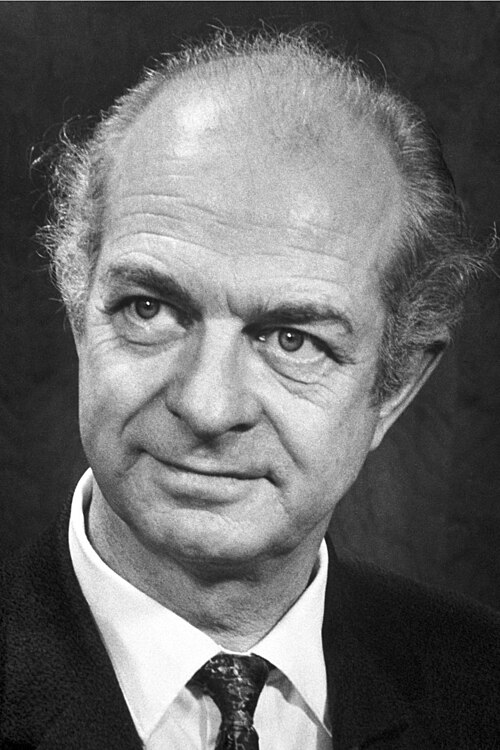
\includegraphics[width=0.24\linewidth]{images/book2/pauling.jpg}

{\small Linus Pauling (1901--1994).}
\end{omfigure}

\section{Tendencias del carácter químico}

\begin{proposition}[Carácter reductor y oxidante]\label{prop:b1:periodicity:redox-trend}
Los elementos de baja energía de ionización y baja \omterm{def:b1:periodicity:electronegativity}{electronegatividad}, a
la izquierda de la tabla y en la parte baja de sus grupos, pierden
electrones con facilidad: son metales reductores (sobre todo los metales
alcalinos). Los elementos de alta \omterm{def:b1:periodicity:electronegativity}{electronegatividad} y alta \omterm{def:b1:periodicity:electron-affinity}{afinidad
electrónica}, arriba a la derecha, ganan electrones con facilidad: son no
metales oxidantes (sobre todo el flúor, el oxígeno y el cloro). Los gases
nobles, con una energía de ionización alta y ninguna afinidad por un
electrón adicional, no hacen ni lo uno ni lo otro.
\end{proposition}

\begin{method}[Predecir una tendencia a partir de la posición]\label{met:b1:periodicity:predict}
Para comparar dos elementos respecto de una propiedad ligada a la fuerza
con que el núcleo retiene los \omterm{def:b1:quantum-numbers:configuration}{electrones de valencia} (radio, $E_i$, $E_{ea}$, $\chi$):
\begin{enumerate}
  \item si están en el mismo grupo, el de más abajo tiene el $n$ mayor:
        radio mayor, $E_i$ y $\chi$ menores;
  \item si están en el mismo \omterm{def:b1:periodicity:table}{periodo}, el de más a la derecha tiene la
        $Z^{*}$ mayor: radio menor, $E_i$ y $\chi$ mayores;
  \item en otro caso, se compara cada uno con el elemento situado en el
        cruce de su fila y la columna del otro;
  \item antes de concluir sobre las energías de ionización, se comprueban
        los efectos de \omterm{def:b1:quantum-numbers:orbital}{subcapa} (comienzo de una \omterm{def:b1:quantum-numbers:orbital}{subcapa} p, primer
        electrón p apareado).
\end{enumerate}
\end{method}

\begin{example}[El litio en una batería]\label{ex:b1:periodicity:lithium}
El litio tiene la \omterm{def:b1:periodicity:electronegativity}{electronegatividad} más baja del \omterm{def:b1:periodicity:table}{periodo} 2 y pierde con
facilidad su electrón 2s, y es además el metal más ligero: transporta la
mayor carga transferible por gramo de todos los elementos, razón por la
que alimenta las baterías recargables. Su \omterm{def:b1:periodicity:ionisation-energy}{primera energía de ionización},
\qty{5.39}{eV}, es mayor que la del sodio (5.14) o la del potasio (4.34)
y, sin embargo, en el agua es el metal alcalino más reductor, una paradoja
que resuelve la fuerte hidratación del pequeño ion \ce{Li+}
(\cref{ch:b1:nernst}).
% ledger: ie:Li, ie:Na, ie:K
\end{example}

\section{Ejercicios}

\begin{exercise}[$\star$]\label{exo:b1:periodicity:1}
Dense el \omterm{def:b1:periodicity:table}{periodo}, el grupo y el \omterm{def:b1:periodicity:table}{bloque} del calcio, el hierro, el selenio
y el yodo ($Z = 20, 26, 34, 53$) a partir de sus configuraciones.
\end{exercise}

\begin{exercise}[$\star$]\label{exo:b1:periodicity:2}
En cada pareja, ¿qué especie es más grande, y por qué? \ce{Na} o
\ce{Cl}; \ce{Na} o \ce{Na+}; \ce{F-} o \ce{Cl-}; \ce{Na+} o \ce{Mg^{2+}}.
\end{exercise}

\begin{exercise}[$\star$]\label{exo:b1:periodicity:3}
Las \omterm{def:b1:periodicity:ionisation-energy}{primeras energías de ionización} de \ce{Na}, \ce{Mg}, \ce{Al}, \ce{P},
\ce{S} y \ce{Ar} son 5.14, 7.65, 5.99, 10.49, 10.36 y
\qty{15.76}{eV}. Ordénense y señálense las dos desviaciones respecto de
la tendencia general.
\end{exercise}

\begin{exercise}[$\star$]\label{exo:b1:periodicity:4}
Defínase la \omterm{def:b1:periodicity:polarisability}{polarizabilidad} de una especie. ¿Cuál es más polarizable,
\ce{F-} o \ce{I-}? ¿\ce{Na+} o \ce{Cl-}? Justifíquese.
\end{exercise}

\begin{exercise}[$\star\star$]\label{exo:b1:periodicity:5}
Las cuatro \omterm{def:b1:periodicity:ionisation-energy}{primeras energías de ionización} de un elemento del \omterm{def:b1:periodicity:table}{periodo} 3
son 5.99, 18.83, 28.45 y \qty{119.99}{eV}. Calcúlense las razones
sucesivas e identifíquense el elemento y el ion que forma.
\end{exercise}

\begin{exercise}[$\star\star$]\label{exo:b1:periodicity:6}
Explíquese por qué el cloro tiene una \omterm{def:b1:periodicity:electron-affinity}{afinidad electrónica} mayor que el
flúor, y por qué el nitrógeno y el magnesio no forman ningún anión
gaseoso estable.
\end{exercise}

\begin{exercise}[$\star\star$]\label{exo:b1:periodicity:7}
Calcúlense las \omterm{def:b1:periodicity:electronegativity}{electronegatividades} de Mulliken del sodio ($E_{i1} =
\qty{5.14}{eV}$, $E_{ea} = \qty{0.55}{eV}$) y del cloro ($E_{i1} =
\qty{12.97}{eV}$, $E_{ea} = \qty{3.61}{eV}$). ¿Qué dicen del enlace en
\ce{NaCl}?
\end{exercise}

\begin{exercise}[$\star\star$]\label{exo:b1:periodicity:8}
Con los valores de Pauling del \cref{ex:b1:periodicity:bonds} y $\chi(\ce{F})
= 3.98$, clasifíquense los enlaces \ce{H-F}, \ce{C-H}, \ce{Na-Cl},
\ce{C-Cl} ($\chi(\ce{Cl}) = 3.16$) y \ce{O-H}, e indíquese el signo de la
carga parcial de cada átomo.
\end{exercise}

\begin{exercise}[$\star\star$]\label{exo:b1:periodicity:9}
Las \omterm{def:b1:periodicity:ionisation-energy}{primeras energías de ionización} de \ce{Li}, \ce{Na} y \ce{K} son
5.39, 5.14 y \qty{4.34}{eV}. Explíquese la tendencia y predígase si la
del rubidio está por encima o por debajo de \qty{4.34}{eV}.
\end{exercise}

\begin{exercise}[$\star\star\star$]\label{exo:b1:periodicity:10}
El cinc ($Z = 30$) tiene una \omterm{def:b1:periodicity:ionisation-energy}{primera energía de ionización} de
\qty{9.39}{eV}, y el galio ($Z = 31$), de \qty{6.00}{eV}; el arsénico
($Z = 33$), de \qty{9.79}{eV}, y el selenio ($Z = 34$), de
\qty{9.75}{eV}. Explíquense las dos caídas a partir de las
configuraciones.
\end{exercise}

\begin{exercise}[$\star\star\star$]\label{exo:b1:periodicity:11}
Tómense $D(\ce{H-H}) = \qty{436}{kJ/mol}$, $D(\ce{F-F}) =
\qty{158}{kJ/mol}$, $\chi(\ce{H}) = 2.20$ y $\chi(\ce{F}) = 3.98$, con
$\qty{1}{eV} = \qty{96.5}{kJ/mol}$. Estímese con la definición de Pauling
la energía de enlace $D(\ce{H-F})$. ¿Por qué es mucho mayor que la media
de los dos enlaces simétricos?
\end{exercise}

\begin{exercise}[$\star\star\star$]\label{exo:b1:periodicity:12}
Las \omterm{def:b1:periodicity:electronegativity}{electronegatividades} de Pauling están tabuladas para el criptón
(3.00) y el xenón (2.60), pero no para el helio, el neón o el argón.
Explíquese, a partir de la definición de la escala, por qué solo puede
darse un valor para un elemento que forma enlaces, y por qué son los
gases nobles más pesados los que los forman.
% ledger: en:Kr, en:Xe
\end{exercise}

\section{Problema: la aritmética de Pauling}

\begin{problem}[{Problema de fin de semana --- un elemento desconocido a
partir de sus energías de ionización, una serie de iones con una nube del
mismo tamaño, dos escalas de electronegatividad y el número de Pauling
para el enlace H--Cl}]
\label{pb:b1:periodicity:1}
Dato: $\qty{1}{eV}$ por partícula corresponde a \qty{96.485}{kJ/mol}.

\medskip
\noindent\textbf{Parte I --- Un elemento desconocido.}
Las cuatro \omterm{def:b1:periodicity:ionisation-energy}{primeras energías de ionización} de un elemento X del \omterm{def:b1:periodicity:table}{periodo} 3
son 7.65, 15.04, 80.14 y \qty{109.27}{eV}.
\begin{enumerate}
  \item ¿Por qué cada energía de ionización es mayor que la anterior?
  \item Calcúlense las razones $E_{i2}/E_{i1}$, $E_{i3}/E_{i2}$ y
        $E_{i4}/E_{i3}$.
  \item Dedúzcase el grupo de X y, después, identifíquese.
  \item ¿Qué ion forma X en sus compuestos? Dese su configuración.
  \item ¿Es X un metal o un no metal? Justifíquese a partir de su posición.
  \item ¿Por qué el tercer electrón cuesta mucho más que el segundo?
\end{enumerate}

\medskip
\noindent\textbf{Parte II --- Diez electrones.}
Los \omterm{def:b1:periodicity:radius}{radios iónicos} (seis vecinos) de \ce{O^{2-}}, \ce{F-}, \ce{Na+},
\ce{Mg^{2+}} y \ce{Al^{3+}} son 140, 133, 102, 72 y \qty{54}{pm}.
\begin{enumerate}[resume]
  \item Demuéstrese que estos iones tienen la misma configuración.
  \item Explíquese el orden de los radios.
  \item ¿Cuál de los cinco iones es el más polarizable, y por qué?
  \item Calcúlese la razón entre el radio mayor y el menor.
  \item La longitud de enlace de \ce{Cl2} es \qty{198.8}{pm}, y el radio
        de \ce{Cl-}, \qty{181}{pm}. Calcúlese el \omterm{def:b1:periodicity:radius}{radio covalente} del cloro
        y compárese.
  \item Sin más datos, ordénense \ce{Cl-}, \ce{Na+} y \ce{Mg^{2+}} por
        tamaño.
\end{enumerate}

\medskip
\noindent\textbf{Parte III --- La \omterm{def:b1:periodicity:electronegativity}{escala de Mulliken}.}
\begin{center}
\small
\begin{tabular}{lccccc}
\hline
elemento & \ce{F} & \ce{Cl} & \ce{Br} & \ce{O} & \ce{C} \\
\hline
$E_{i1}$ (eV) & 17.42 & 12.97 & 11.81 & 13.62 & 11.26 \\
$E_{ea}$ (eV) & 3.40 & 3.61 & 3.36 & 1.44 & 1.26 \\
$\chi$ de Pauling & 3.98 & 3.16 & 2.96 & 3.44 & 2.55 \\
\hline
\end{tabular}
\end{center}
% ledger: ie:F, ie:Cl, ie:Br, ie:O, ie:C, ea:F, ea:Cl, ea:Br, ea:O, ea:C,
% en:F, en:Cl, en:Br, en:O, en:C
\begin{enumerate}[resume]
  \item Calcúlense las \omterm{def:b1:periodicity:electronegativity}{electronegatividades} de Mulliken de los cinco
        elementos.
  \item Ordénense en cada escala. ¿Qué elemento ocupa un lugar distinto?
  \item Calcúlese la razón $\chi_{\text{Pauling}}/\chi_M$ para los tres
        halógenos. ¿Qué se observa?
  \item Propóngase por qué el oxígeno se aparta de la regla de los
        halógenos (obsérvese su \omterm{def:b1:periodicity:electron-affinity}{afinidad electrónica}).
  \item ¿Qué átomo lleva la carga parcial negativa en \ce{HCl}? ¿Y en
        \ce{ClF}?
  \item Con los valores tabulados ($\chi(\ce{H}) = 2.20$), ¿el enlace
        \ce{H-Cl} es apolar, covalente polar o iónico?
\end{enumerate}

\medskip
\noindent\textbf{Parte IV --- El número de Pauling para H--Cl.}
Las entalpías estándar de formación de \ce{H(g)}, \ce{Cl(g)} y
\ce{HCl(g)} a \qty{298}{K} son 218.0, 121.3 y \qty{-92.3}{kJ/mol}; las de
\ce{H2(g)} y \ce{Cl2(g)} son nulas. La energía de enlace de una molécula
se toma igual a la entalpía de su disociación en átomos.
% ledger: janaf:H, janaf:Cl, janaf:HCl
\begin{enumerate}[resume]
  \item Calcúlese $D(\ce{H-H})$ a partir de \ce{H2(g) -> 2H(g)}.
  \item Calcúlese $D(\ce{Cl-Cl})$.
  \item Calcúlese $D(\ce{H-Cl})$ a partir de \ce{HCl(g) -> H(g) + Cl(g)}.
  \item Calcúlese la energía en exceso de Pauling, $\Delta E$, en kJ/mol,
        y demuéstrese que es igual a $-\Delta_f H(\ce{HCl})$.
  \item Conviértase $\Delta E$ en electronvoltios.
  \item Calcúlese $|\chi(\ce{Cl}) - \chi(\ce{H})|$ y compárese con la
        diferencia de los valores tabulados, $3.16 - 2.20$.
\end{enumerate}
\end{problem}
